Final states with two same-sign leptons or three leptons and multiple jets are sensitive to a variety of new physics scenarios. 
In supersymmetric models in particular, such final states can be produced 
in the decays of heavy superpartners involving massive gauge bosons, sleptons or top quarks. 
Depending on the nature of the particles accompanying the leptons in the final states, 
a large variety of signatures can be obtained, notably in terms of the numbers of jets and $b$-tagged jets in the final state. 
We chose to illustrate the analysis versatility by evaluating its sensitivity to 
six $R$-parity-conserving (RPC) SUSY scenarios with the lightest neutralino \neut\ as lightest and stable superpartner, 
featuring gluino, bottom squark or top squark pair production. 
The first scenarios studied focus on gluino pair production with decays into on-shell (Figure~\ref{fig:feynman_gtt}) 
or off-shell (Figure~\ref{fig:feynman_gttOffshell}) top quarks, as well as on-shell light quarks. The latter are accompanied by a cascade decay involving 
a $\chinoonepm$ and a $\ninotwo$ (Figure~\ref{fig:feynman_gg2WZ}) or a $\ninotwo$ and light sleptons (Figure~\ref{fig:feynman_gg2sl}). 
The other two scenarios target the direct production of third-generation squark pairs 
with subsequent electroweakino-mediated decays (Figures~\ref{fig:feynman_b1b1} and~\ref{fig:feynman_t1t1}). 
The former is characterized by final states with bottom squark pairs decaying to $\ttbar WW\ninoone\ninoone$. The latter, addressed here by 
looking at a final state with three same-sign leptons, is a model that could explain the excess seen in same-sign lepton signatures 
during Run~1~\cite{Huang:2015fba}.
Finally, a full SUSY model with low fine-tuning, the non-universal Higgs model with two extra parameters (NUHM2)~\cite{Ellis:2002iu,Ellis:2002wv}, 
is also considered. When the soft-SUSY-breaking electroweakino mass, $m_{1/2}$, is in the range 300--800 GeV, the model mainly 
involves gluino pair production with gluinos decaying predominantely 
to $\ttbar\ninoone$ and $tb\chinoonepm$, giving rise to final states with two same-sign leptons and \met.

\begin{figure}[t!]
\centering
\begin{tabular}{rrrr}
\subfloat[]{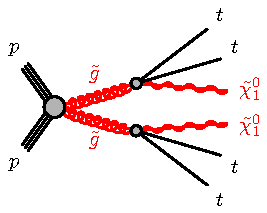
\includegraphics[width=0.24\textwidth]{gogo-ttttN1N1}\label{fig:feynman_gtt}} &
\subfloat[]{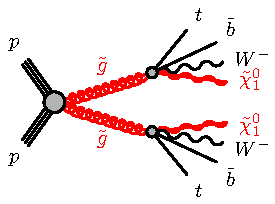
\includegraphics[width=0.24\textwidth]{gogo-ttWWbbN1N1}\label{fig:feynman_gttOffshell}} &
\subfloat[]{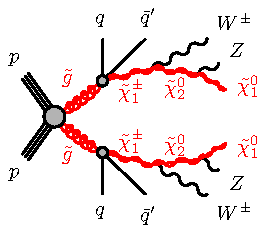
\includegraphics[width=0.24\textwidth]{gogo-qqqqWWZZN1N1-C1N2}\label{fig:feynman_gg2WZ}} &
\subfloat[]{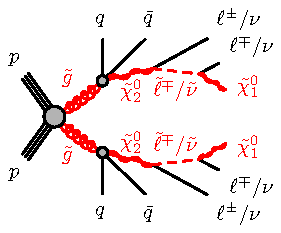
\includegraphics[width=0.24\textwidth]{gogo-qqqqllllN1N1-N2}\label{fig:feynman_gg2sl}}  \\
&
\subfloat[]{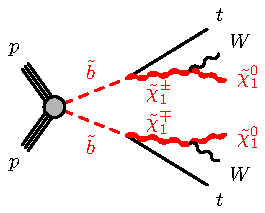
\includegraphics[width=0.24\textwidth]{sbsb-ttWWN1N1}\label{fig:feynman_b1b1}} &
\subfloat[]{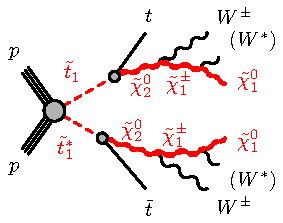
\includegraphics[width=0.24\textwidth]{stst-ttWWWWN1N1}\label{fig:feynman_t1t1}} & 
 \\
\end{tabular}
\caption{SUSY processes featuring gluino ((a), (b), (c), (d)) or third-generation squark ((e), (f)) pair production studied in this analysis. 
 In Figure~\ref{fig:feynman_gg2sl}, $\tilde{\ell} \equiv \tilde{e}, \tilde{\mu}, \tilde{\tau}$ and 
$\tilde{\nu} \equiv \tilde{\nu}_e, \tilde{\nu}_{\mu}, \tilde{\nu}_{\tau}$. In Figure~\ref{fig:feynman_t1t1}, the $W^*$ labels indicate 
largely off-shell $W$ bosons -- the mass difference between $\chinoonepm$ and $\ninoone$ is around 1~GeV.}
\label{fig:feynman}
\end{figure}

These scenarios were used as benchmarks to identify regions of the phase space 
where the analysis can bring particularly useful complementarity to other SUSY 
searches, 
and subsequently define our signal regions with a particular focus on these 
regions. 
In this section, the scenarios considered are presetend with details about 
the assumed superpartner masses and decay modes.  
Exclusion limits obtained prior to the work of the author will also 
be shown to highlight the improvement in reach after the current analysis.


\begin{figure}[t]
\centering
\subfloat[]{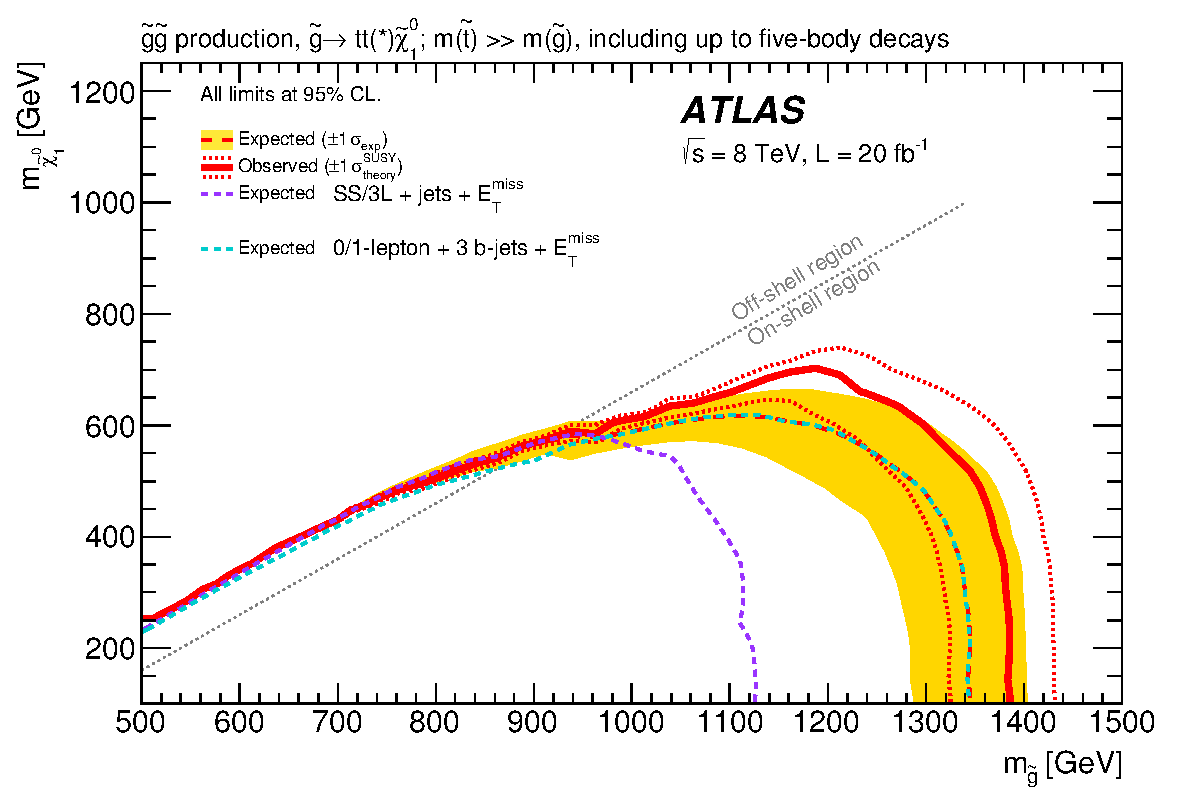
\includegraphics[width=0.55\textwidth]{run1excluded_gluinoGtt}}
\subfloat[]{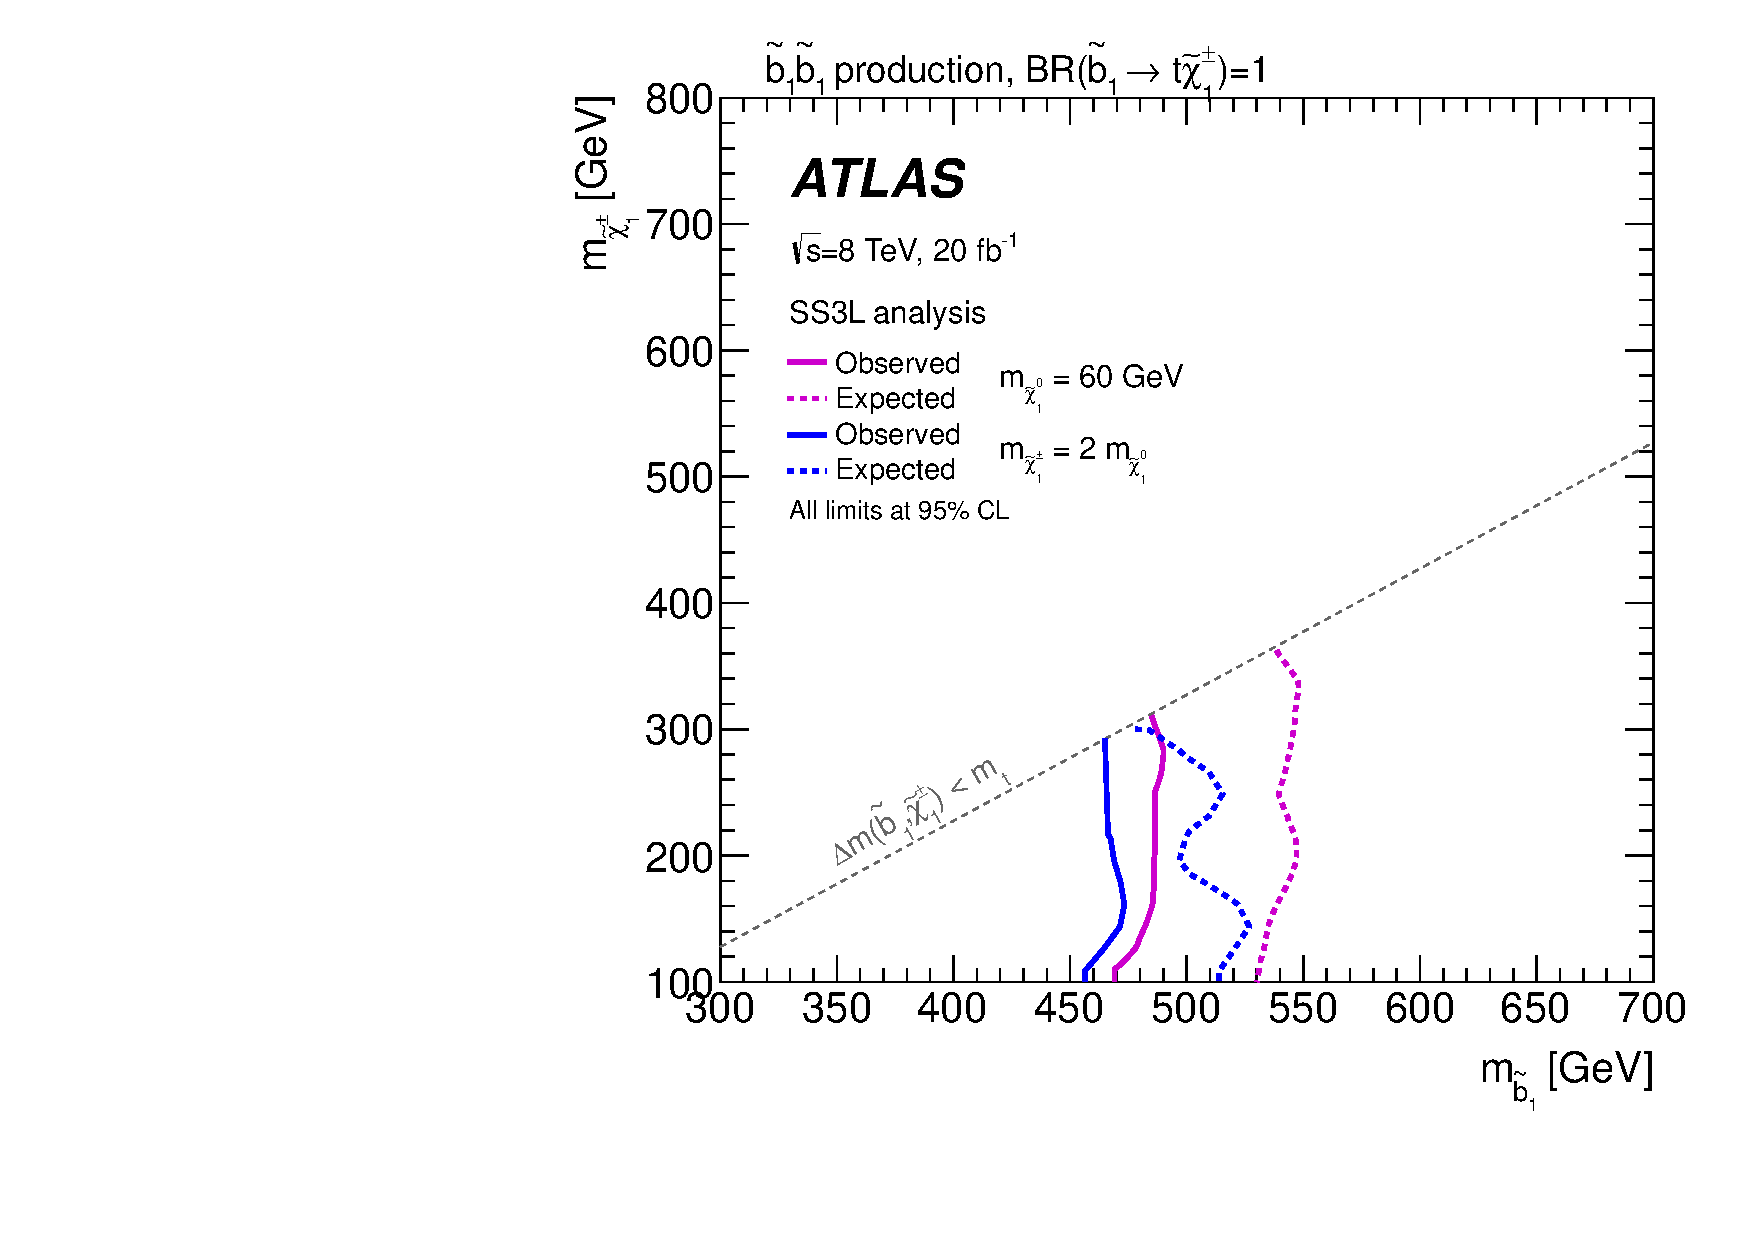
\includegraphics[width=0.38\textwidth]{exclusion_sbottom_topC1_both_grids}}
\caption{Exclusion limits on the gluino-stop offshell (left) and direct sbottom (right) scenarios 
set by ATLAS with the 2012 dataset~\cite{DraftSquarkGluinoSummaryPaper}
prior to the author's work.}
\label{fig:run1excl_3rdgen}
\end{figure}


\begin{figure}[t]
\centering
\subfloat[]{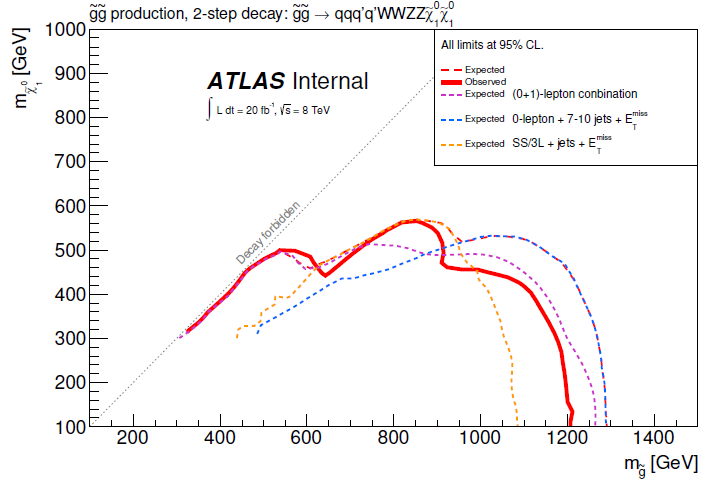
\includegraphics[width=0.49\textwidth]{run1excluded_gluino2stepWZ}}
\subfloat[]{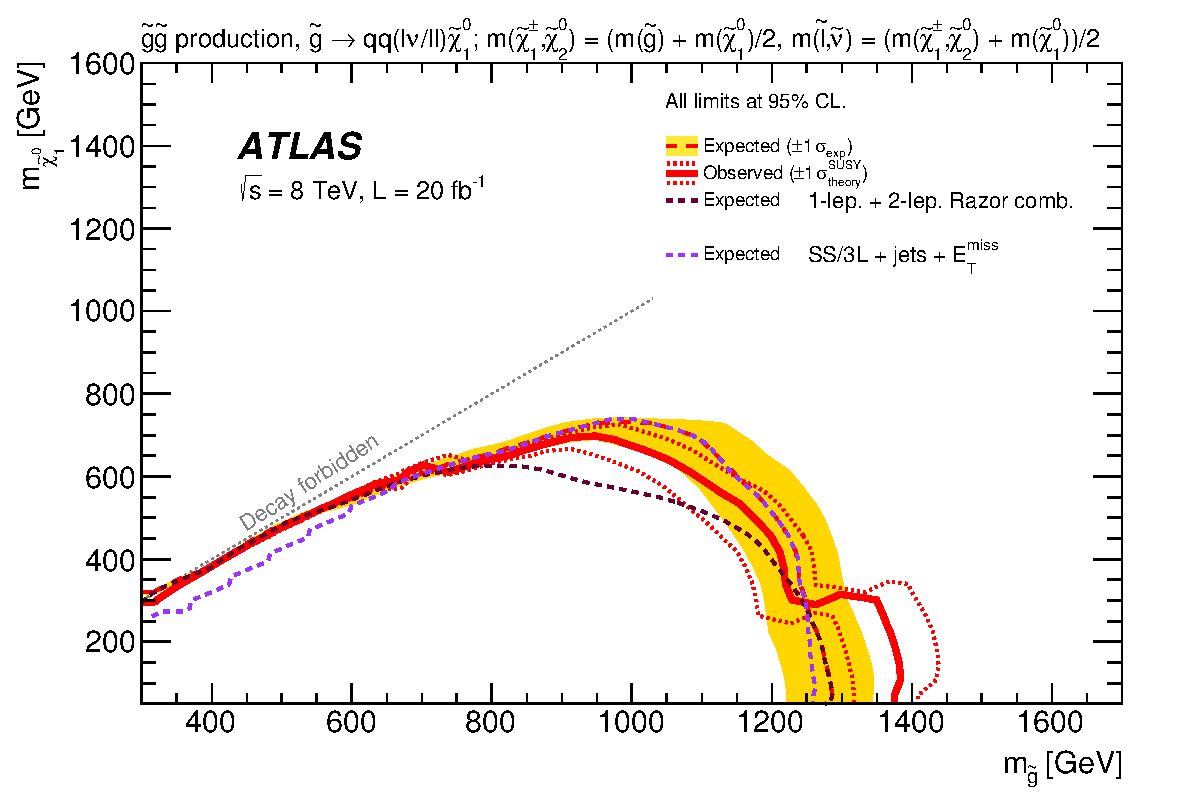
\includegraphics[width=0.49\textwidth]{run1excluded_gluino2stepSleptons}}
\caption{Exclusion limits on scenarios featuring gluino pair production followed by two-step decays via heavy gauge bosons or sleptons, 
set by ATLAS with the 2012 dataset~\cite{DraftSquarkGluinoSummaryPaper}
prior to the author's work.}
\label{fig:run1excluded_1stgen}
\end{figure}

\subsection{Gluino pair production with slepton-mediated two-step decay $\gl\to q\bar q\ell\bar\ell\neut$}
\label{subsec:signals_g2slep}

This scenario (Fig.~\ref{fig:feynm_g2slep}) features gluino pair-production with two-step decays via neutralinos \neuttwo\ and sleptons, 
$\gl\to q\bar{q}'\neuttwo \to q\bar{q}'(\slep\ell/\snu\nu) \to q\bar{q}'(\ell\ell/\nu\nu)\neut$. 
The decays are mediated by generic heavy squarks, therefore the $b$-jet multiplicity in this scenario is low. 
The final state is made of charged leptons, four additional jets and invisible particles (neutrinos and neutralinos). 
The average jet multiplicity per event is the smallest among the four scenarios;  
another characteristic is the large fraction of events with several leptons, 
unlike the other scenarios that have a rather low acceptance due to the branching ratios of $W\to\ell\nu$ or $Z\to\ell\ell$. 
The exclusion limits obtained in run-1 (Fig.~\ref{fig:run1excluded_1stgen} right) show again that the SS/3L+jets final state 
is very competitive to probe those models. 
This scenario is used as as benchmark to define the signal regions with $\ge 3$ leptons and no $b$-jet. 

The signal grid is built with variable gluino and \neut\ masses; the \neuttwo\ mass is chosen half-way between the gluino and LSP masses, 
and the sleptons masses are also set equal and half-way between the \neuttwo\ and LSP masses. 
The \neuttwo\ may decay to any of the six ``left-handed'' sleptons (\slep, \snu) with equal probability. 
``Right-handed'' sleptons are assumed heavy and do not participate to the decay. 
%% The generated MC samples assume equiprobable mediation of the decay through all (mass-degenerate) squarks except top squarks, 
%% which can lead to final states with several $b$-jets in case of sbottom-mediated decays. 
%% However, we veto such decays and reweight other events by a factor $1/(2*0.2*0.8+0.2^2)$ to readjust the branching ratios, 
%% effectively modifying the model assumptions such that only decays mediated by the four light-flavour squarks occur. 
%% This is done in order to simplify the model description (the other scenario, described in the next section, doesn't have sbottom-mediated decays), 
%% as well as respect the motivation of this scenario, to be a guideline for the definition of $b$-depleted signal regions. 


\subsection{Gluino pair production with gaugino-mediated two-step decay $\gl\to q\bar q'WZ\neut$}
\label{subsec:signals_g2wz}

This scenario (Fig.~\ref{fig:feynm_g2wz}) features gluino pair-production with two-step decays via gauginos and $W$ and $Z$ bosons, 
$\gl\to q\bar{q}'\chargino\to q\bar{q}'W\neuttwo\to q\bar{q}'WZ\neut$, 
mediated by generic heavy squarks of the first and second generations. 
The final state is made of two $W$ and two $Z$ bosons (possibly offshell), 
four additional jets and invisible particles (neutrinos and neutralinos). 
This generally leads to events with large jet multiplicities and a fair branching ratio for dileptonic final states. 
The exclusion limits obtained in run-1 indeed illustrate the competitiveness of the SS/3L+jets search (Fig.~\ref{fig:run1excluded_1stgen} left)
particularly the heavy-\neut\ region of the phase space. 
This scenario is used as as benchmark to define the signal regions with many jets but none tagged as a $b$-jet. 

The signal grid is built with variable gluino and \neut\ masses, 
and the \chargino\ and \neuttwo\ masses are set such that the former lies half-way between the gluino and \neut\ masses, 
and the latter half-way between \chargino\ and \neut\ masses. 

\subsection{Sbottom pair production with one-step decay $\sbot\to t\chargino$}
\label{subsec:signals_sbot}

In this scenario (Fig.~\ref{fig:feynm_sbot}), bottom squarks are rather light and assumed to decay in a top quark and a chargino $\chargino$, 
with a subsequent $\chargino\to W^\pm\neut$ decay, 
providing complementarity to the mainstream search~\cite{ATLAS-CONF-2015-066} which focuses on the channel $\sbot\to b\neut$. 
The final state resulting from the production of a \sbsb\ pair contains two top quarks, two $W$ bosons and two neutralinos. 
While this final state may lead to various experimental signatures, 
the model was considered in Run-1~\cite{DraftSquarkGluinoSummaryPaper} 
only by the same-sign leptons and jets search, leading to the exclusion limits presented in Fig.~\ref{fig:run1excl_3rdgen}. 
Signal events typically contain one or two $b$-tagged jets, 
therefore this scenario is used as benchmark to define the signal regions with $\ge 1$ $b$-jet. 

The model adopts a fixed chargino-neutralino mass difference of 100 GeV, 
therefore always allowing on-shell $W$ bosons in the $\chargino\to W\neut$ decay
\footnote{A different chargino mass assumption is adopted in the current 
work compared to the Run-1 paper~\cite{DraftSquarkGluinoSummaryPaper}.
Fig.~\ref{fig:run1excl_3rdgen} is shown for illustration only.
The reduced chargino-neutralino mass gap in the current analysis 
allows to study signal scenarios with heavy neutralinos, which were not considered previously.}
Only pair production of the lightest sbottom is considered, followed by an exclusive decay in the aforementioned channel. 


\subsection{Gluino pair production with stop-mediated decay $\gl\to t\bar t\neut$}
\label{subsec:signals_gtt}

In this scenario inspired by naturalness arguments, gluinos are coupling preferentially to stops which are lighter than the other squarks. 
Gluinos are however considered lighter than stops, and decay directly into a $t\bar t\neut$ triplet via a virtual stop (Fig.~\ref{fig:feynm_gtt}). 
The pair production of gluinos leads to a final state containing four top quarks and two neutralinos. 
This characteristic final state is accessible through various experimental signatures, which is why this model 
is commonly used as a benchmark to compare analyses sensitivities. 
The searches performed with Run-1 data~\cite{DraftSquarkGluinoSummaryPaper}, 
summarized in Fig.~\ref{fig:run1excl_3rdgen}, showed that the same-sign leptons final state is competitive only at large neutralino mass. 
This region of the phase space is consequently given a particular attention in the choice of signal regions described further on. 
For instance, the region of phase-space with $\Delta m(\gl,\neut)<2m_t$, where gluinos decay via one or two offshell top quarks, is only accessible for this 
analysis.
In the signal samples referenced in this document, the mass of the lightest stop is fixed to 10 \TeV and is mostly a $\widetilde{t}_R$ state. 
Only gluino pair production is considered, followed by an exclusive decay in the aforementioned channel. 
Signal events typically contain many $b$-tagged jets, 
therefore this scenario is used as benchmark to define the signal regions with $\ge 2$ $b$-jets. 

\subsection{\stst\ with ``three-same-sign leptons'' signature}
\label{subsec:signals_3lss}

Inspired by Ref.~\cite{stop_3lss}, a simplified model featuring a stop pair-production with two-step 
decays via a neutralino \neuttwo\ and a chargino $\chargino$ is added in this version of the analysis, according to the decay illustrated on 
Fig.~\ref{fig:feynm_stop}: \\
$\stop_1\to t \neuttwo \to t \chargino W^\mp \to t W^\pm W^\mp \neut$. 

This simplified model is a well-motivated representation of a pMSSM model. 
The lightest stop ($\stop_1$) is right-handed and \neuttwo\ is bino-like 
which leads to a large branching ratio in the decay $\stop_1\to t \neuttwo$. 
Furthermore, the decay $\neuttwo \to \chargino W^\mp$ is also enhanced since $\chargino$ is wino-like, 
as long as $\chargino$ and \neut~ are nearly mass degenerate 
and $m_{\neuttwo} - m_{\neut} < m_{H} = 125 \GeV$ to suppress the decay $\neuttwo \to \neut + H$ 
(the decay $\neuttwo \to \neut + Z$ is suppressed).
By respecting these conditions and evading the bottom squark limit shown in Fig.~\ref{fig:limitsSummer_rpc}, c, we consider
 a one-dimensional grid with a $\stop_1$ mass varying between 550 \GeV and 800 \GeV with a 50 \GeV gap\footnote{Only the points at $\stop_1$ mass of 550~GeV are available at the moment.}, 
a two body decay to an on-shell top quark and a \neuttwo~ which has a 100 \GeV mass difference from \neut.
The mass difference between the $\chargino$ and \neut~ is taken to be 500 \MeV which is not excluded by the disappearing track 
analysis. In fact, this mass gap could easily be increased by introducing a small amount of higgsino mixing~\cite{Aad:2013di}.
%  https://atlas.web.cern.ch/Atlas/GROUPS/PHYSICS/PAPERS/SUSY-2013-01/fig_07.png

While the stop pair production is similar to the sbottom pair production in terms of kinematics, the stop pair production offers 
a unique topology that leads to three leptons of the same electric charge. This final state benefits from an extreme reduction of 
the SM background while maintaining a good signal acceptance which helps loosen the kinematic cuts to access a more compressed 
SUSY phase space. As a result, this scenario is complementary to the search for bottom squarks.


\subsection{Non-Universal Higgs Models}
\label{subsec:signals_nuhm2}

In references~\cite{Baer:2013xua,Baer:2013yha,Baer:2016usl}, 
theorists studied a complete two-extra-parameter non-universal Higgs model (NUHM2) 
that can have low fine tuning (natural) and
predicts final state signatures that allow large background rejection while retaining high 
signal efficiency. 
The NUHM2 model allows the soft SUSY breaking masses of the Higgs multiplets, $m_{H_{u}}$ and $m_{H_{d}}$, to be different from 
matter scalar masses ($m_{0}$) at the grand unification scale. The NUHM2 model is expected to form the effective theory for energies 
lower than $m_{GUT}$ resulting from SU(5) or general SU(10) grand unified theories.
The scalar mass $m_{0}$, the soft SUSY breaking gaugino mass $m_{1/2}$, the pseudoscalar Higgs boson mass $m_{A}$, the trilinear SUSY breaking parameter $A_{0}$, the weak scale ratio of Higgs field vacuum expectation values $\tan\beta$, and the superpotential Higgs mass $\mu$ are the free parameters.
Both $m_{1/2}$ and $\mu$ are varied while the other parameters are fixed to $m_{0} = 5$ TeV, $A_{0} = -1.6m_{0}$, $\tan\beta = 15$, $m_{A} = 1$ TeV, and sign($\mu$)$>$0. 
These parameter choices lead directly to a Higgs mass of 125~GeV in accord with experiment.  In this ``radiatively-driven natural'' SUSY approach, the higgsino is
required to have mass below 200-300~GeV, the stop to have a mass below
$\sim$3~TeV, and the gluino below $\sim$4~TeV.
Final state topologies that include MET, $W \to \ell\nu$ and 
that result in same-sign dileptons can be explored. 
Simulated NUHM2 signal samples with mass $(m_{1/2})$ values from 300-800 GeV and $\mu = 150$ GeV were generated.
The gluino mass in this model is approximately $2.5\times m_{1/2}$.
Table~\ref{tab:NUHM2} shows the branching ratios of the dominant gluino decay modes for $m_{1/2} = 400$ GeV.

\begin{table}[t!]
\begin{center}
\begin{tabular}{|c|c||c|c|}
\hline
\hline
Decay & BR & Decay & BR\\
\hline
$t\bar{t}\chi^{0}_{1}$ & 0.13 & $tb\chi^{\pm}_{1}$ & 0.45\\
$t\bar{t}\chi^{0}_{2}$ & 0.21 & $tb\chi^{\pm}_{2}$ & 0.04\\
$t\bar{t}\chi^{0}_{3}$ & 0.13 & - & - \\
$t\bar{t}\chi^{0}_{4}$ & 0.02 & - & - \\
\hline
$t\bar{t}\chi^{0}_{i}$ & 0.49 & $tb\chi^{\pm}_{i}$ & 0.49\\
\hline
\hline
\end{tabular}
\caption{The dominant gluino decay modes for $m_{1/2} = 400$ GeV for the NUHM2 model.}
\label{tab:NUHM2}
\end{center}
\end{table}

\subsection{Signal cross-sections and simulations}
\label{subsec:signals_simulation}

\begin{table}[t!]
\centering
\caption{Signal cross-sections [pb] and related uncertainties [\%] for scenarios featuring \glgl\ (top table) or \sbsb\  (bottom table) production, 
as a function of the pair-produced superpartner mass, reproduced from Ref.~\cite{twiki-SusyCrossSections}.}
\label{tab:signal_xsections}
\resizebox{\textwidth}{!}{
\begin{tabular}{|c|c|c|c|c|c|c|c|c|c|c|}
\hline\hline
Gluino mass (GeV) & 500 & 550 & 600 & 650 & 700 \\\hline
Cross section (pb) & $27.4 \pm 14\%$ & $15.6 \pm 14\%$ & $9.20 \pm 14\%$ & $5.60 \pm 14\%$ & $3.53 \pm 14\%$\\\hline\hline
750 & 800 & 850 & 900 & 950 & 1000\\\hline
$2.27 \pm 14\%$ & $1.49 \pm 15\%$ & $0.996 \pm 15\%$ & $0.677 \pm 16\%$ & $0.466 \pm 16\%$ & $0.325 \pm 17\%$\\\hline\hline
1050 & 1100 & 1150 & 1200 & 1250 & 1300\\\hline
$0.229 \pm 17\%$ & $0.163 \pm 18\%$ & $0.118 \pm 18\%$ & $0.0856 \pm 18\%$ & $0.0627 \pm 19\%$ & $0.0461 \pm 20\%$\\\hline\hline
1350 & 1400 & 1450 & 1500 & 1550 & 1600\\\hline
$0.0340 \pm 20\%$ & $0.0253 \pm 21\%$ & $0.0189 \pm 22\%$ & $0.0142 \pm 23\%$ & $0.0107 \pm 23\%$ & $0.00810 \pm 24\%$\\\hline\hline
\end{tabular}}

\resizebox{0.8\textwidth}{!}{
\begin{tabular}{|c|c|c|c|c|}
\hline\hline
Sbottom mass (GeV) & 400 & 450 & 500 & 550 \\\hline
Cross section (pb) & $1.84 \pm 14\%$ & $0.948 \pm 13\%$ & $0.518 \pm 13\%$ & $0.296 \pm 13\%$\\\hline\hline
600 & 650 & 700 & 750 & 800\\\hline
$0.175 \pm 13\%$ & $0.107 \pm 13\%$ & $0.0670 \pm 13\%$ & $0.0431 \pm 14\%$ & $0.0283 \pm 14\%$\\\hline\hline
\end{tabular}}
\end{table}

The signal processes are generated from leading order (LO) matrix elements with up to two extra partons (only one for the grid featuring slepton-mediated gluino decays), 
using the \textsc{Madgraph v5.2.2.3} generator~\cite{Alwall:2014hca} interfaced to \textsc{Pythia} 8.186~\cite{Sjostrand:2007gs} 
with the \textit{ATLAS 14} tune~\cite{ATL-PHYS-PUB-2014-021} for the modelling of the SUSY decay chain, parton showering, 
hadronisation and the description of the underlying event. 
For the RPV models, \textsc{Madgraph v5.2.3.3} and \textsc{Pythia} 8.210~\cite{Sjostrand:2007gs} were used instead. 
Parton luminosities are provided by the \textsc{NNPDF23LO}~\cite{Carrazza:2013axa} set of parton distribution functions. 
Jet-parton matching is realized following the CKKW-L prescription~\cite{Lonnblad:2011xx}, 
with a matching scale set to one quarter of the pair-produced superpartner mass. 

The signal samples are normalised to the next-to-next-to-leading order cross-section from Ref.~\cite{twiki-SusyCrossSections} 
including the resummation of soft gluon emission at next-to-next-to-leading-logarithmic accuracy (NLO+NLL), 
as detailed in Ref.~\cite{Borschensky:2014cia}; 
some of these cross-sections are shown for illustration in Table~\ref{tab:signal_xsections}. 
For the production of like-sign d-squark (RPV scenario), 
Prospino~\cite{Beenakker:1996ed} is used to scale the samples to their NLO cross-section.

Cross-section uncertainties are also taken from Ref.~\cite{twiki-SusyCrossSections} as well, 
and include contributions from varied normalization and factorization scales, as well as PDF uncertainties. 
They typically vary between 15 and 25\%. 
We do not consider any source of uncertainties on signal acceptance, 
experience having shown that these are generally smaller than the uncertainties on the inclusive production cross-section. [this is currently being verified for some cases]

The dataset IDs are listed in appendix~\ref{app:samples}, Table~\ref{tab:SigSamples}, 
and further details on simulation and reconstruction are provided in section~\ref{subsubsec:samples_mc}. 
